
\documentclass{manufacturing21conf}

% ============================================================
% NOTE SYSTEM FOR DRAFTING (cor, modi, acl)
%
% This document uses three custom inline note commands
% based on the "todonotes" package. They allow the author
% to insert comments directly in the text while writing.
%
% Commands:
%   \cor{...}   → marks a Correction needed
%   \modi{...}  → marks a Modification or suggested change
%   \acl{...}   → marks a Clarification or explanation for the author
%
% Example:
%   This sentence is unclear. \cor{Rewrite this part.}
%   \modi{Consider adding a reference here.}
%   \acl{We discussed this idea in Section 2.}
%
% SHOW / HIDE NOTES:
%   To show notes during drafting:
%       \shownotestrue
%
%   To hide all notes in the final PDF:
%       \shownotesfalse
%
% When notes are hidden, the commands produce no output.
% You do NOT need to remove them manually from the text.
%
% ============================================================

% ---------------------------------------------------------
% TITLE + AUTHORS
% ---------------------------------------------------------
\title{Comparative Evaluation of Chatter Detection Indicators under Simulated Machining Conditions}

% Usa \affil{a}, \affil{b} como definimos en el .sty
\author{
  Enrique MIRELES HERNANDEZ \affil{a, b},\ 
  Mikhail GUSKOV \affil{a},\
  Philippe LORONG \affil{a},\
  Théo Dorlin \affil{b},\
  Habib KARAOUNI \affil{b}
}

\affiliations{
  \affilLine{(a) Laboratoire PIMM, Arts et Metiers Institude of Technology, 151 boulevard de l'Hopital, 75013 Paris, France}
  \affilLine{(b) Safran S.A., Research \& Technology Center, F-78772 Magny-les-Hameaux, France}
}


\email{Mail : \textcolor{blue}{enrique.mireles\_hernandez@ensam.eu}}



% % ---------------------------------------------------------
% % TABLE EXAMPLE
% % ---------------------------------------------------------
% \begin{table}[ht]
%   \caption{Example table caption}
%   \label{tab:example}
%   \begin{tabular}{lccccc}
%     Ti & Al & Mo & V & Cr \\
%     82 & 5  & 5  & 5 & 3  \\
%   \end{tabular}
% \end{table}

% % ---------------------------------------------------------
% % FIGURE EXAMPLE
% % ---------------------------------------------------------
% \begin{figure}[ht]
%   \centering
%   % Dummy figure
%   \fbox{\rule{0pt}{3cm}\rule{5cm}{0pt}}
%   \caption{Example figure caption}
%   \label{fig:example}
% \end{figure}

% % ---------------------------------------------------------
% % EQUATION EXAMPLE
% % ---------------------------------------------------------
% \begin{equation}\label{eq:heat}
%   \rho C_p \frac{\partial T}{\partial t}
%   - \nabla(K \nabla T) = \omega'_{\text{heat}}
% \end{equation}

\shownotestrue      % show notes while drafting
% \shownotesfalse   % hide notes in final version



\begin{document}

\maketitle





% ---------------------------------------------------------
% ABSTRACT
% ---------------------------------------------------------
\begin{abstractM21}
Early detection of chatter would potentially enable reducing surface degradation, tool wear, and machine tool degradation. While numerous time- and frequency-domain indicators exist, their relative sensitivity and robustness are rarely assessed under a unified framework. This work presents a systematic benchmark of chatter detection indicators using controlled time-domain simulations of machining dynamics. The study compares representative approaches based on vibration energy trends, phase space geometry, statistical signal descriptors, and other time-domain features, including a novel energy based indicator. All methods are tested within identical simulation conditions and signal processing settings. The evaluation focuses on three aspects: the earliest detectable sign of instability, robustness to measurement noise, and consistency across varying cutting parameters. The resulting performance map provides insight into how different indicators respond to chatter onset and under what conditions they remain reliable. The study aims to clarify the trade-offs among existing methods and to guide the selection of effective, real-time or offline chatter detection strategies for stable and productive machining operations.
\end{abstractM21}

% ---------------------------------------------------------
% KEYWORDS (entorno sin argumentos)
% ---------------------------------------------------------
\begin{keywordsM21}
Chatter detection, Early detection, Time-domain simulation, Indicator benchmarking, Signal processing, Machining stability, 
\end{keywordsM21}

% ---------------------------------------------------------
% MAIN CONTENT
% ---------------------------------------------------------



% ---------------------------------------------------------
%               INTRODUCTION
% ---------------------------------------------------------
\section{Introduction}


Chatter is a self-excited vibration that arises when the tool–workpiece interaction enters an unstable regime dominated by regenerative effects and machine structural dynamics \parencite{Quintana2011, Altintas2012_A4}. It increases forces and displacements, degrades accuracy and surface finish, and can lead to tool breakage or spindle damage \parencite{Zhu2020}. Chatter occurs in conventional milling and turning as well as in low-stiffness configurations such as robotic machining, where structural flexibility amplifies instability \parencite{Wang2016_RoboticBoring_A5}. Despite extensive work on dynamic models and stability diagrams \parencite{AltintasBudak1995_A4}, the time-varying and nonlinear nature of cutting limits purely analytical prediction under realistic conditions, motivating online monitoring within TCM and intelligent-machine frameworks \parencite{Li2017}.

Several signal sources have been exploited for chatter detection, including structural vibration, cutting force, and radiated sound \parencite{ Delio1992Audio}. Acoustic sensors are non-intrusive and low-cost, whereas cutting force directly reflects the tool–workpiece interaction. The goal is not only to identify fully developed chatter but to detect as early as possible the transition from stable cutting to incipient slight chatter, where regenerative oscillations start to grow while remaining masked by noise and forced excitation \parencite{Yang2019_A3}. Such early detection is especially critical in high-speed machining and low-stiffness systems \parencite{Zhu2020} and motivates algorithms able to classify the process state online under noisy, non-stationary conditions \parencite{Chen2019}. Existing methods are usually grouped into four families: time-domain indicators (e.g. RMS, kurtosis, cycle energy), frequency-domain approaches based on FFT or spectral density \parencite{Tangjitsitcharoen2013_A4}, time–frequency techniques such as STFT, wavelets, or Hilbert–Huang, and machine-learning approaches using features from vibration, force, or sound \parencite{ Cao2017_Early_A3}.

However, strong heterogeneity in machines, structural stiffness, tools, materials, cutting parameters, noise levels, and signal-processing pipelines hinders fair comparison and generalization across studies \parencite{Nath2020}, and reliable detection of slight chatter embedded in noise remains an open problem \parencite{Tansel2010_TorqueIBR_A5}. In this context, there is still no unified comparative framework assessing, under controlled and reproducible conditions, the ability of different indicators to detect chatter onset. The present work addresses this gap through a systematic benchmark based on time-domain simulations. Unlike studies focused on a single method and configuration \parencite{Zhou2018}, multiple indicators are compared here on identical signals, cutting conditions, and noise levels. The set includes representative time-domain, statistical, time–frequency, and energy-based metrics, together with a novel phase-space-area indicator tailored to slight chatter. All indicators are evaluated with a common protocol that quantifies their sensitivity to early instability, robustness to measurement noise, and consistency under varying cutting parameters, yielding a comparative performance map of their behaviour around chatter onset.


% ---------------------------------------------------------
% MODELING OF MACHINING DYNAMICS
% ---------------------------------------------------------
\section{Time-domain cutting model and simulation campaign}
\acl{Objectif: Expliquer d'ou on obtient les donne}

\subsection{Dynamic cutting model}

The simulated signals are obtained from a classical regenerative cutting model \parencite{Altintas2012_A4}. 
The cutting setup is shown in \figref{fig:sistema}, and the theoretical stability lobes in \figref{subfig:Nessy2m_SLD}. 
The simulation parameters are listed in \tabref{tab:modal_parameters}.


\begin{figure}[ht]
  \centering
  \begin{subfigure}[t]{0.40\textwidth}
    % \centering
    % \includegraphics[height=4cm, keepaspectratio]{Images/Cono.pdf_tex}
    \centering
    \begingroup
    \huge
    \resizebox{!}{4cm}{%
      \import{Images/}{Cono.pdf_tex}%
    }
    \endgroup
    % \caption{Subfigura A}
    % \label{subfig: A}
  \end{subfigure}
  \hfill
  \hspace{1.5cm}
  \begin{subfigure}[t]{0.35\textwidth}
    \centering
    \includegraphics[height=4cm, keepaspectratio]{Images/Sistema_Forces.pdf}
    % \caption{Subfigura B}
    % \label{subfig: B}
  \end{subfigure}
  \caption{Two-degrees-of-freedom (2-DOF) system for dynamic simulations,
used to generate Stability Lobe Diagrams (SLD).}
  \label{fig:sistema}
\end{figure}



The tool-workpiece dynamics are modelled with a single vibration mode and a linear cutting-force law acting on the instantaneous chip thickness. The system is therefore governed by
\begin{equation}
  m \ddot x(t) + c \dot x(t) + k x(t)
  = K_f a(t) \,\bigl[h_0 + x(t-T) - x(t)\bigr],
  \label{eq:eom_single}
\end{equation}

\begin{table}[h!]
\centering
\caption{\textit{Modal parameters used in the simulation.}}
  \begin{tabular}{cccccc}
  \hline
  Mode & $\omega_n$ (Hz) & $\zeta$ (\%) & $k$ (N/m) & $m$ (kg) & $\theta$ (degree) \\
  \hline
  $x_1$ & 250 & 1.2 & $2.26 \times 10^8$ & 9.57 & 30$^\circ$ \\
  $x_2$ & 150 & 1.0 & $2.13 \times 10^8$ & 15.48 & 60$^\circ$ \\
  \hline
  \end{tabular}
  \label{tab:modal_parameters}
\end{table}

% a compact formulation that captures the essential regenerative mechanism leading to chatter.




% ================================================
\subsection{Numerical implementation}

All signals are generated with the machining simulator \emph{Nessy2m}, which provides  tool-tip displacement, velocity, and force for the cutting setup shown in \figref{subfig:Nessy2m_setup}.  A single scenario is used: a depth-of-cut ramp from 5~mm to 15~mm at 120{,}000~rpm and  0.05~mm/tooth (feed rate 6000~mm/min). The sampling rate ensures 200 samples per  revolution (400~kHz), and the total duration is 15~s.

Only the dominant 150~Hz mode is activated, and no measurement noise is added. Most 
indicators use the velocity signal, while the proposed phase-space energy indicator 
requires both displacement and velocity.

\begin{figure}[ht]
  \centering
  \begin{subfigure}[t]{0.40\textwidth}
    \centering
    % \includegraphics[height=4cm, keepaspectratio]{Images/Nessy2m_Piece.png}
    \begingroup
    \huge
    \resizebox{!}{4cm}{%
      \import{Images/}{Nessy2m_Piece.pdf_tex}%
    }
    \endgroup
    \caption{Nessy2m simulation setup}
    \label{subfig:Nessy2m_setup}
  \end{subfigure}
  % \hfill
  \hspace{1cm}
  \begin{subfigure}[t]{0.40\textwidth}
    \centering
    \includegraphics[height=4cm, keepaspectratio]{Images/SLD.pdf}
    \caption{SLD for the 2-DOF system}
    \label{subfig:Nessy2m_SLD}
  \end{subfigure}
  \caption{Nessy2m simulation setup and corresponding Stability Lobe Diagram (SLD).}
  \label{fig:Nessy2m_setup_full}
\end{figure}




\subsection{Simulation campaign}

A single high-resolution time-domain simulation is used for all indicators to ensure 
a fair and fully controlled comparison. The depth-of-cut ramp provides a smooth 
transition from stable cutting to regenerative instability, with the stability limit 
crossed at approximately $h_{lim} = 8.6052$~mm \figref{subfig:Nessy2m_SLD} around $t_E = 7.32$~s (Section \ref{subsec:reference_regions}). This allows all indicators to  be evaluated on the same, well-defined chatter onset. Each method is therefore tested  under identical conditions using exactly the same vibration signal.

\acl{Objectif: Decrire les indicateurs qu'on va tester}
% ================================
% 3. CHATTER INDICATORS
% ================================

\section{Chatter indicators considered in this benchmark}

A minimal but representative set of chatter indicators is selected to cover the main
mechanisms linked to early instability. All methods are applied to the same tool-tip
velocity signal $v(t)$ under a unified comparison protocol. Only the essential
functional definitions are reported here; full algorithmic details can be found in the original references.



% =========================================
% 3.1 EMD-Hilbert indicator
% =========================================
\subsection{EMD--Hilbert indicator (force-based surrogate)}

This indicator isolates high-frequency content that becomes excited as chatter develops. First, empirical mode decomposition (EMD) extracts $\mathrm{IMF}_1$, the intrinsic mode concentrating the highest frequencies in $v(t)$. Regenerative chatter injects energy into a specific frequency band, causing $\mathrm{IMF}_1$ to grow. The Hilbert transform produces the analytic signal, from which the instantaneous amplitude and Hilbert spectrogram are derived. Chatter manifests as an increasing number of instantaneous-amplitude points within the predefined chatter-sensitive band. The progression is: raw signal $\rightarrow$ IMF isolation $\rightarrow$ Hilbert analytic signal $\rightarrow$ instantaneous amplitude in chatter band \parencite{Wang2018_RoboticBoring_EMD}.
\medskip
\[
\underbrace{\mathrm{IMF}_1(t)=\mathrm{EMD}\{v(t)\}_1}_{\text{Mode extraction}}
\,\longrightarrow\,
\underbrace{z_1(t)=\mathrm{IMF}_1(t)+i\,\mathcal{H}\{\mathrm{IMF}_1(t)\}}_{\text{Hilbert analytic signal}}
\,\longrightarrow\,
\underbrace{I_{\mathrm{EMD}}(t)=|z_1(t)|}_{\substack{\text{Instantaneous amplitude}\\[2pt]\text{in chatter band}}}.
\]

% =========================================
% 3.2 MaxEnt-SPRT indicator
% =========================================
\subsection{MaxEnt--SPRT indicator (cycle-based probabilistic)}

This indicator transforms the vibration into progressively richer statistical representations. A once-per-revolution (OPR) value $v_k$ captures cycle-to-cycle behavior directly influenced by regenerative dynamics. The maximum entropy (MaxEnt) of short OPR segments quantifies the spread of the distribution, which increases during slight chatter. The sequential probability ratio test (SPRT) then accumulates deviations relative to a baseline stable model. An essential offline calibration phase determines the MaxEnt probability densities for stable $p_0(\mathrm{ME})$ and incipient-chatter $p_1(\mathrm{ME})$ conditions \parencite{Zhao2019_MaxEnt}.
\medskip
\[
\underbrace{v_k = v(t_k)}_{\text{OPR sample}}
\,\longrightarrow\,
\underbrace{\mathrm{ME}(k) = -\!\int f_k(v)\ln f_k(v)\,dv}_{\text{MaxEnt (cycle dispersion)}}
\,\longrightarrow\,
\underbrace{I_{\mathrm{SPRT}}(n)=\sum_{k=1}^{n}\ln\!\left[\frac{p_1(\mathrm{ME}(k))}{p_0(\mathrm{ME}(k))}\right]}_{\text{Sequential indicator (cumulative evidence)}}.
\]

% =========================================
% 3.3 SST-SVD indicator
% =========================================
\subsection{SST--SVD indicator (synchrosqueezed time--frequency energy)}

This indicator reveals chatter by progressively refining the spectral structure of the vibration signal. First, the Synchrosqueezing Transform (SST) sharpens the time--frequency (TF) representation. Second, spindle- and tooth-passing harmonics are removed to expose energy growth near structural frequencies. Third, the filtered TF map is decomposed via SVD: (1) construct the TF window, (2) compute its singular value spectrum, and (3) track the largest singular value. In the original formulation, detection relies on a $3\sigma$ threshold, requiring a stable segment to estimate mean and variance \parencite{Cao2016_Synchrosqueezing}.
\medskip
\[
\underbrace{T_v(f,t)=\mathrm{SST}\{v(t)\}}_{\text{Sharpened TF map}}
\,\longrightarrow\,
\underbrace{T_v^{\mathrm{filt}}(f,t)}_{\substack{\text{TPF}\\\text{harmonic removal}}}
\,\longrightarrow\,
\underbrace{(U,D,V)=\mathrm{SVD}\big(T_v^{\mathrm{filt}}(\cdot,t_i)\big)}_{\text{TF decomposition}}
\,\longrightarrow\,
\underbrace{I_{\mathrm{SST}}(t_i)=D_{11}}_{\substack{\text{Dominant TF energy}\\\text{(chatter growth)}}}.
\]
% =========================================
% 3.4 CV indicator
% =========================================
\subsection{Coefficient of Variation (CV)}

This indicator measures normalized amplitude variability. The velocity signal is transformed into a sliding-window RMS sequence, capturing envelope fluctuations. As chatter develops, the RMS values become increasingly irregular. The CV normalizes this variability and provides a simple and robust instability metric. Each new RMS value is computed by discarding the oldest sample and adding the newest one \parencite{Ye2018_CoV}.
\medskip
\[
\underbrace{v_{\mathrm{RMS}}(k)=\sqrt{\tfrac{1}{N}\sum_{i=1}^{N}v_i^2}}_{\text{Envelope extraction (sliding window)}}
\,\longrightarrow\,
\underbrace{I_{\mathrm{CV}}=\tfrac{\mathrm{std}(v_{\mathrm{RMS}})}{\mathrm{mean}(v_{\mathrm{RMS}})}}_{\text{Normalized variability}}.
\]

% =========================================
% 3.5 Phase-space spiral-area indicator
% =========================================
\subsection{Phase-space spiral-area indicator (proposed)}

This indicator evaluates the mechanical energy flow in the phase-space trajectory $(x(t),v(t))$. A sliding observation window containing five complete oscillation cycles is used. For each cycle, the spiral area quantifies net energy exchange: areas shrink when damping dominates (stable cutting) and expand when regenerative feedback injects energy (incipient chatter). The logarithmic decrement between consecutive areas captures the energy-growth rate \parencite{Hernandez2025_EarlyChatter}.
\medskip
\[
\underbrace{
A_j=\tfrac12\sum_{\ell}(x_\ell v_{\ell+1}-x_{\ell+1}v_\ell)
}_{\text{Cycle energy (spiral area)}}
\,\longrightarrow\,
\underbrace{
\delta_j=-\ln\!\left(\tfrac{A_{j+1}}{A_j}\right)
}_{\text{Energy-growth rate}}
\,\longrightarrow\,
\underbrace{I_{\mathrm{phase}}(t_k)=\delta^{(k)}
}_{\substack{\text{Instability indicator}\\\text{over five cycles}}}.
\]





% ---------------------------------------------------------
% Benchmark protocol and performance metrics
% ---------------------------------------------------------
\section{Benchmark protocol and performance metrics}
\acl{Objectif: Expliquer comment on va evaluer les indicateurs}


\subsection{Ground truth and reference regions}
\label{subsec:reference_regions}

\subsubsection{\texorpdfstring{Linear stability boundary and $t_E$}{Linear stability boundary and tE}}


The ground truth is obtained from the linearised regenerative 1-DOF model \ecref{eq:eom_single}.  
Linear perturbations $x(t)=X e^{\lambda t}$ lead to the characteristic equation
\begin{equation}
\label{eq:char}
m\lambda^2 + c\lambda + k + K_f a(t)\bigl(1-e^{-\lambda T}\bigr)=0.
\end{equation}

At each instant, the dominant root $\lambda_{\max}(a(t))$ is extracted and its real part
\begin{equation}
\label{eq:sigma}
\sigma(t)=\Re\{\lambda_{\max}(a(t))\}
\end{equation}
is evaluated numerically.

The time at which the system crosses the stability boundary is defined as
\begin{equation}
\label{eq:tE}
t_E:\qquad \sigma(t_E)=0,\qquad \sigma(t)<0\ \forall\, t<t_E .
\end{equation}

\subsubsection{\texorpdfstring{Amplitude growth and $t_{\text{vis}}(R)$}{Amplitude growth and t\_vis(R)}}

After $t_E$, the vibration envelope satisfies
\begin{equation}
\label{eq:env}
A(t) \approx A(t_E)\exp\bigl(G(t)\bigr), 
\qquad 
G(t)=\int_{t_E}^{t}\sigma(\tau)\,d\tau .
\end{equation}

The visibility time $t_{\text{vis}}(R)$ is defined as the first instant where the accumulated growth reaches
\begin{equation}
\label{eq:tvis}
G\!\left(t_{\text{vis}}(R)\right)=\ln R ,
\end{equation}
providing a noise-free, dynamics-based visibility threshold.

Under the depth-of-cut ramp $a(t)=a_{p,0}+\dot a_p t$, the times 
$t_E$ and $t_{\text{vis}}(R)$ correspond to depths $a_E$ and $a_{\text{vis}}$ on the stability diagram. Both $t_E$ and $t_{\text{vis}}(R)$ are model-based references common to all indicators.
 

\subsubsection{\texorpdfstring{Visibility levels $R$}{Visibility levels R}}

Three levels are used:
\begin{itemize}[nosep,leftmargin=1.8em]
    \item $R=3$ (+9.5 dB): very early chatter,
    \item $R=5$ (+14 dB): intermediate growth,
    \item $R=10$ (+20 dB): clearly visible chatter.
\end{itemize}
The dependence of $t_{\text{vis}}(R)$ on $R$ remains moderate due to the slow variation of $\sigma(t)$.

% ================================================


\subsubsection{Temporal regions}

Using $t_E$ and $t_{\text{vis}}(R)$, the benchmark timeline is partitioned into
\begin{subequations}\label{eq:regions}
\begin{align}
\mathcal{R}_{\mathrm{st}}      &= [t_{\mathrm{st},1},\, t_{\mathrm{st},2}],
&\text{(strictly stable: } t<t_E\text{)}, 
\label{eq:Rst} \\[0pt]
\mathcal{R}_{\mathrm{EC}}(R)   &= [t_E,\, t_{\text{vis}}(R)],
&\text{(early chatter: } t_E \le t \le t_{\text{vis}}(R)\text{)}, 
\label{eq:REC} \\[0pt]
\mathcal{R}_{\mathrm{ch}}(R)   &= [t_{\text{vis}}(R),\, t_{\mathrm{end}}],
&\text{(developed chatter: } t>t_{\text{vis}}(R)\text{)}.
\label{eq:Rch}
\end{align}
\end{subequations}

False alarms are evaluated in $\mathcal{R}_{\mathrm{st}}$ and 
early detections in $\mathcal{R}_{\mathrm{EC}}(R)$.



% ================================================

\subsubsection{Dimensionless time and normalised detection index}

A unified time scale is introduced as
\begin{equation}
\xi(t)=\frac{t-t_E}{t_{\text{vis}}(R)-t_E},
\end{equation}
where $\xi=0$ corresponds to the stability boundary and $\xi=1$ to the chosen visibility level.  
If an indicator triggers at $t_d$, its normalised index is
\begin{equation}
\eta=\xi(t_d).
\end{equation}
Interpretation: $\eta<0$ (premature), $0<\eta<1$ (early chatter), $\eta>1$ (late).  
This normalisation removes scale, smoothing and unit dependence, enabling direct comparison across heterogeneous indicators.

% \subsubsection{Illustrative ground-truth plot (optional)}

% Figure~X illustrates $\sigma(t)$, $G(t)$, the times $t_E$, $t_{\text{vis}}(R)$, and the three temporal regions.

% ================================================
\subsection{Unified comparison layer and detection time}

Each indicator retains its native formulation, but all decision rules are 
anchored to the strictly stable region $\mathcal{R}_{\mathrm{st}}$, which 
provides a method-specific stable baseline.  Indicators whose original 
design already relies on this notion (SST--SVD via its $3\sigma$ envelope, 
MaxEnt--SPRT via $p_0$) are used as published.  For CV, EMD--Hilbert and 
the spiral-area ratio, the values observed in $\mathcal{R}_{\mathrm{st}}$ 
define respectively a reproducible CV threshold, a stable energy level, 
and a zero-drift trend for the logarithmic area ratio.  Chatter is declared 
when the indicator departs persistently from its baseline according to its 
native decision logic.  This yields comparable detection times $t_d$ 
without modifying the intrinsic behaviour of any method.

\subsection{Performance metrics}

Using the normalised time $\xi(t)$ and detection index $\eta$, four
quantities characterise each indicator.

\textbf{Detection delay.}
$\eta$ provides the primary sensitivity measure
($\eta<0$ premature, $0<\eta<1$ early, $\eta>1$ late).  
Absolute delay: $\Delta t = t_d - t_E$.

\textbf{False alarms.}
With activations $\mathcal{A}$ in the strictly stable region 
$\mathcal{R}_{\mathrm{st}}=[t_{\mathrm{st},1},t_{\mathrm{st},2}]$,
\begin{equation}
\mathrm{FAR}
=\frac{|\mathcal{A}\cap\mathcal{R}_{\mathrm{st}}|}{|\mathcal{R}_{\mathrm{st}}|}.
\end{equation}

\textbf{Stable-region variability.}
For the raw indicator $I(t)$,
\begin{equation}
\sigma^2_{\mathrm{st}}
=\mathrm{Var}\!\left(I(t);\;t\in\mathcal{R}_{\mathrm{st}}\right),
\qquad
\delta_{\mathrm{st}}
=\max_{t\in\mathcal{R}_{\mathrm{st}}}|I(t)-\bar I_{\mathrm{st}}|.
\end{equation}

\textbf{Early-chatter slope.}
Responsiveness across $\mathcal{R}_{\mathrm{EC}}=[t_E,t_{\mathrm{vis}}(R)]$ is
\begin{equation}
\gamma
=\frac{I(t_{\mathrm{vis}})-I(t_E)}{t_{\mathrm{vis}}-t_E}.
\end{equation}

These metrics compactly quantify sensitivity, false alarms, and baseline
stability under a unified time scale.




% ---------------------------------------------------------
% RESULTS 
% ---------------------------------------------------------
\section{Results }


% ---------------------------------------------------------
% DISCUSSION
% ---------------------------------------------------------
\section{Discussion }


% ---------------------------------------------------------
% CONCLUSION
% ---------------------------------------------------------
\section{Conclusion and outlook }

% ---------------------------------------------------------
% ACKNOWLEDGMENTS
% ---------------------------------------------------------
\begin{acknowledgmentsM21}
The authors would like to thank their collaborators and sponsors for 
supporting this research effort.
\end{acknowledgmentsM21}

% ---------------------------------------------------------
% REFERENCES
% ---------------------------------------------------------
% \begin{thebibliography}{1}

% \bibitem{Lee1951}
% E.~H. Lee, B.~W. Schaeffer (1951) The theory of plasticity applied to a
% problem of machining, \textit{Journal of Applied Mechanics}, vol.~18,
% pp.~405--413.

% \end{thebibliography}

\printbibliography[title={References}]

\end{document}
